\chapter{評価}
\label{chap:evaluation}

本章では、本研究における評価手法とその結果について述べる。

\section{評価手法}

\ref{chap:implementation}章で実装したAES67送受信アプリケーションを使用する。2台のPCでそれぞれ送信機能と受信機能を動作させ、伝送にかかる遅延時間を計測する。

\section{評価環境}

コンピュータを2台、ネットワークスイッチを介して接続する。その構成を、それぞれ表\ref{tab:evaluation_computer}と表\ref{tab:evaluation_network}に示す。接続図\ref{fig:evaluation_environment}に示した。

\begin{figure}[tbp]
  \centering
  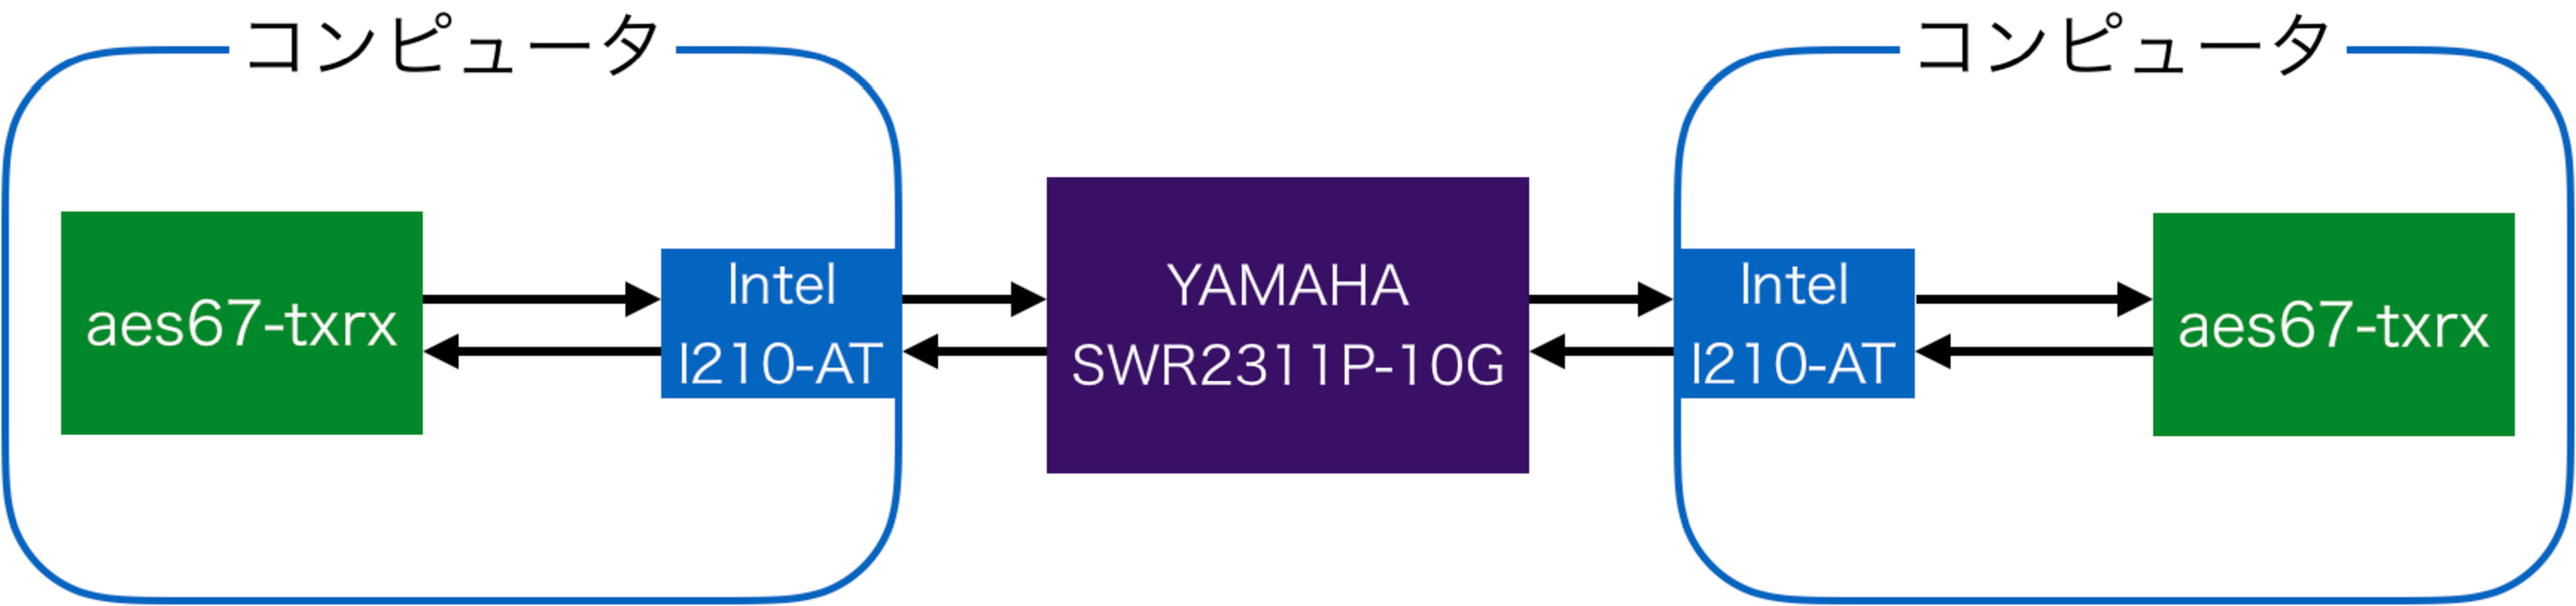
\includegraphics[width=\linewidth]{img/evaluation_environment.pdf}
  \caption{評価環境の接続図}
  \label{fig:evaluation_environment}
\end{figure}

今回使用するネットワークスイッチは、Dante最適設定が搭載されている。使用機材のヤマハ SWR2311P-10Gのドキュメント\cite{yamaha-swr2311p-dante}によると、Dante最適設定では、安定したIPオーディオ伝送を行うための以下の設定がネットワークスイッチに書き込まれる。

\begin{itemize}
  \item システム全体
  \begin{itemize}
    \item フロー制御を無効
    \item QoSを有効
    \item DSCP値による送信キューの最適化
  \end{itemize}
  \item VLANインターフェース
  \begin{itemize}
    \item IGMPスヌーピングを有効
    \item IGMPクエリー送信機能を有効
    \item IGMPクエリー送信間隔の設定
    \item IGMPパケットのTTL値検証機能を無効
  \end{itemize}
  \item LAN/SFPポート
  \begin{itemize}
    \item QoSトラストモードをDSCPに設定
    \item フロー制御を無効
    \item EEEを無効
  \end{itemize}
\end{itemize}

Dante最適設定を有効にした状態で計測を行った。

\begin{table}[tbp]
  \caption{コンピュータ評価環境}
  \label{tab:evaluation_computer}
  \centering
  \begin{tabular}{c|l} \hline
    OS & Ubuntu 18.04 LTS (Linux 5.3.0-28-generic)\\ \hline
    CPU & Intel Core i7-9700K 3.60GHz \\ \hline
    RAM & 32GB \\ \hline
    SSD & Samsung SSD 970 EVO Plus 250GB \\ \hline
    NIC & StarTech ST1000SPEXI (Intel I210-AT) \\ \hline
  \end{tabular}
\end{table}

\begin{table}[tbp]
  \caption{ネットワーク評価環境}
  \label{tab:evaluation_network}
  \centering
  \begin{tabular}{c|l} \hline
    ネットワークスイッチ & YAMAHA SWR2311P-10G \\ \hline
  \end{tabular}
\end{table}

\section{AES67伝送の結果}

\subsection{RTPストリームパケット送受信時間}

\begin{figure}[tbp]
  \centering
  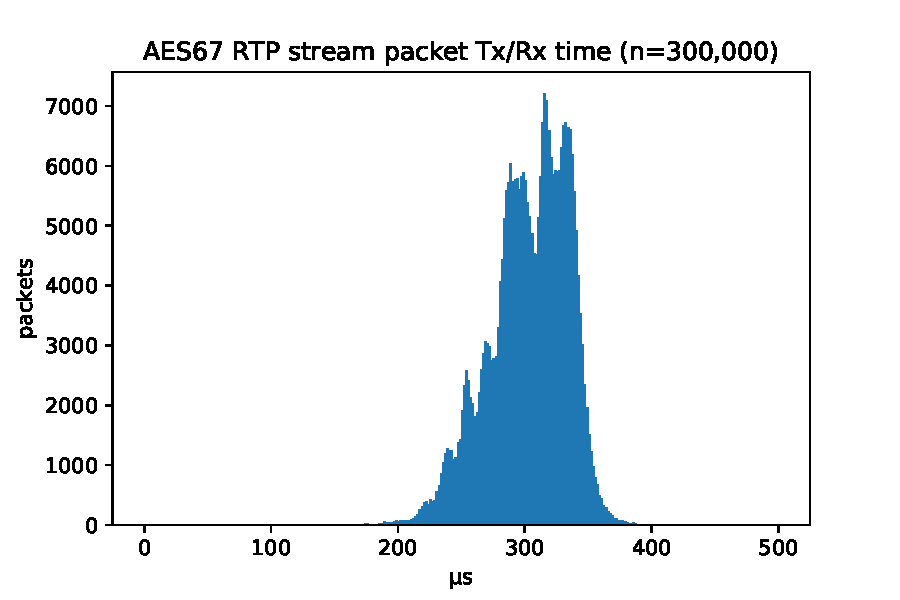
\includegraphics[width=\linewidth]{img/packets_graph.pdf}
  \caption{AES67のRTPストリームパケット送受信時間}
  \label{fig:packets_graph}
\end{figure}

RTPストリームパケット送受信にかかる時間は、最小91.125マイクロ秒、最大3490.794マイクロ秒、平均303.402マイクロ秒、中央値306.710マイクロ秒であった(小数点以下4桁を四捨五入)。

そのうち、1ミリ秒を超えるものは8回、2ミリ秒を超えるものは2回あった。

\subsection{パケットロス率}

パケットロス率は、0\%だった。

\section{追加実験}

前述したパケット送受信の実験はAES67伝送にかかる時間を計測した。当初の目的である、AES67オーディオシステムにかかわるすべての処理が\ref{sec:pro_audio_requirement}節で述べた20ミリ秒以内に収まるのかを検証するため、さらに次の実験を行った。

\subsection{追加実験の概要}

この実験は、アナログ・デジタル変換(A/D)、デジタル・アナログ変換(D/A)にかかる時間を計測し、AES67のRTPストリームパケット送受信にかかる時間と合わせて20ミリ秒以内になるかを検証するものである。

実験に用いた機材と接続の構成を図\ref{fig:advance_test}に示す。

\begin{figure}[tbp]
  \centering
  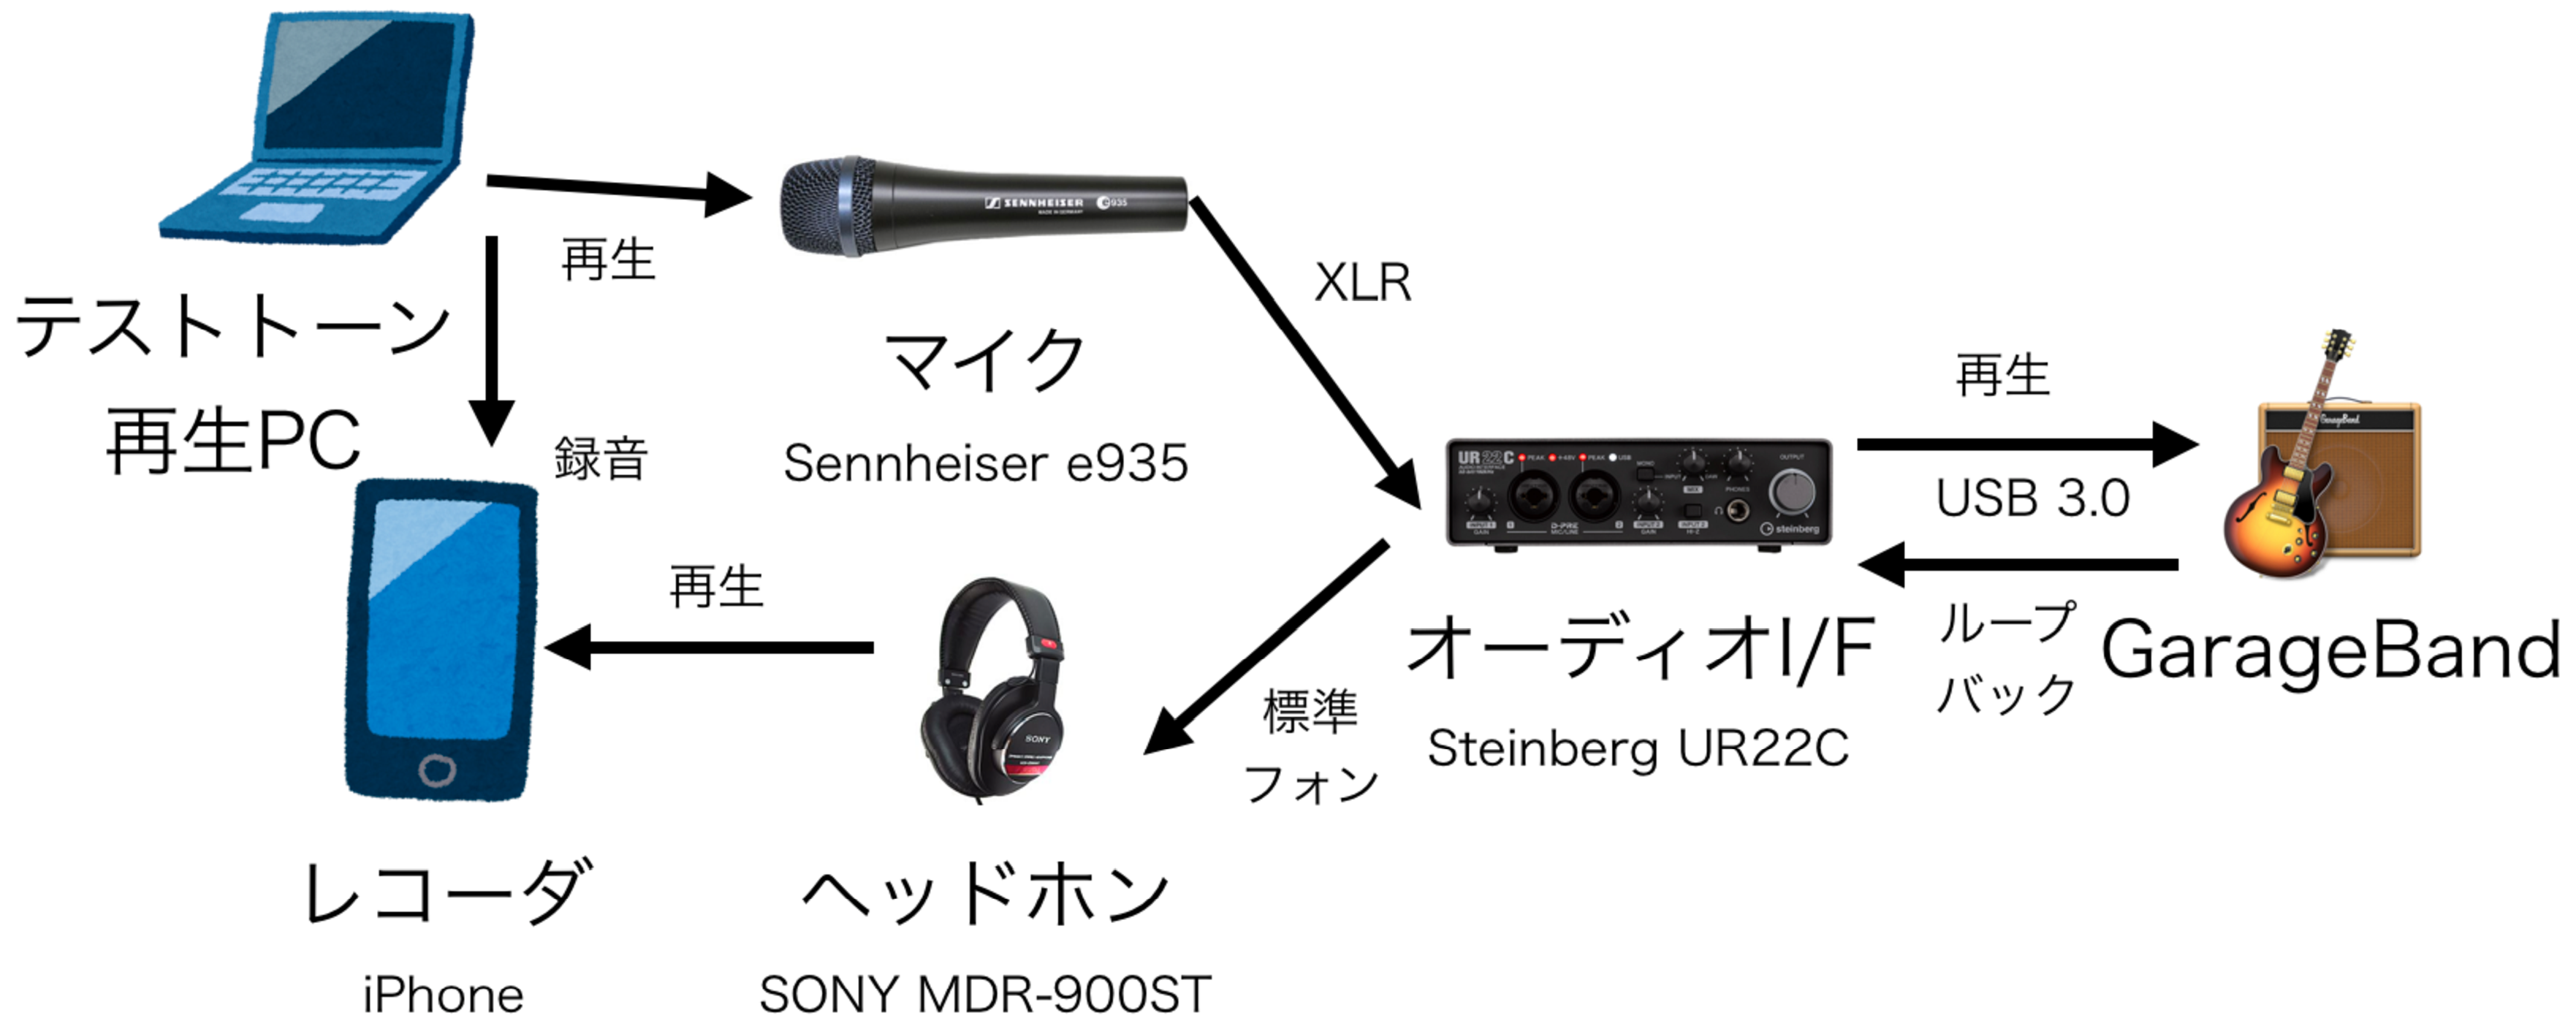
\includegraphics[width=\linewidth]{img/advance_test.pdf}
  \caption{追加実験環境の接続図}
  \label{fig:advance_test}
\end{figure}

実験に用いるオーディオは、オープンソースのオーディオエディタであるAudacity\footnote{\url{https://www.audacityteam.org/}}を用いてテストトーンを生成する。1kHzのサイン波トーンを、500マイクロ秒で48kHz、24bitのオーディオを再生する。

\subsection{追加実験の結果}

\begin{figure}[tbp]
  \centering
  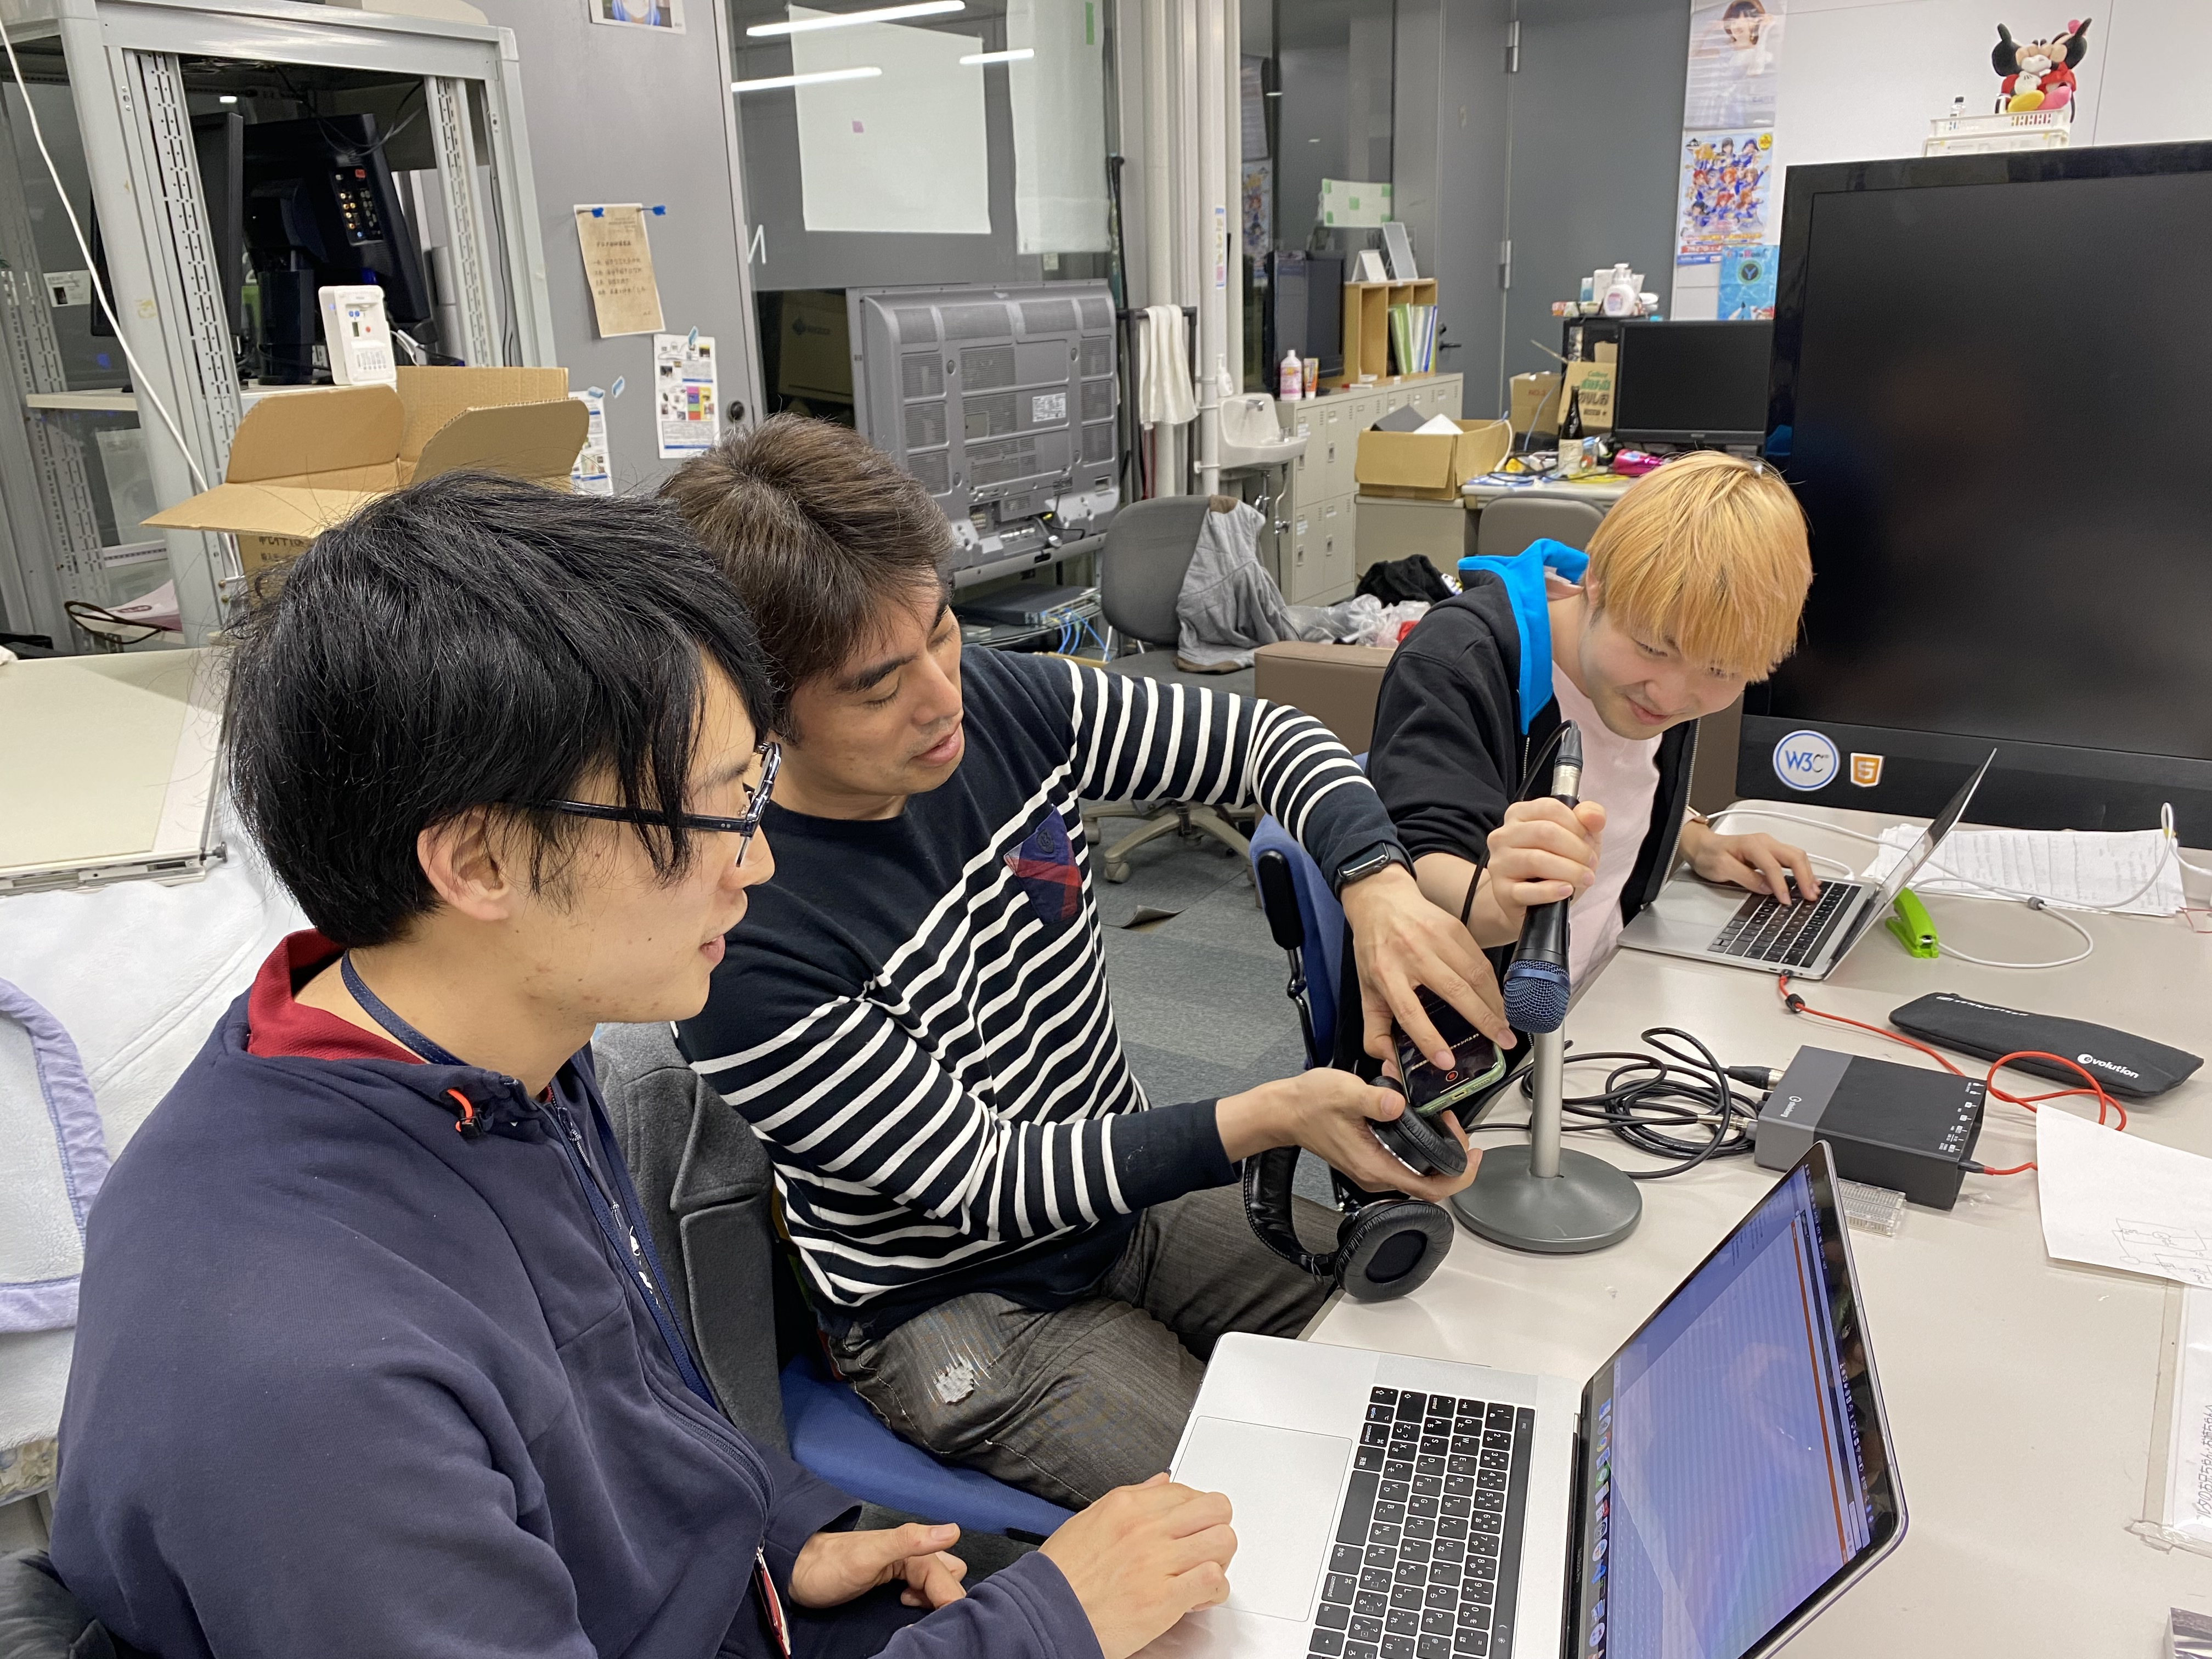
\includegraphics[width=\linewidth]{img/advance_test_people.jpg}
  \caption{追加実験を行う様子}
  \label{fig:advance_test_people}
\end{figure}

テストトーンを再生したPCと、オーディオインターフェイスのモニター端子に接続したヘッドホンの音を録音したファイルをAudacityで開いた。図\ref{fig:advance_test_monitor}にその結果を示す。

図\ref{fig:advance_test_monitor}において、上段のオーディオはテストトーンを再生しモニターに出力した状態、下段はテストトーンを再生するのみでモニターに出力したい状態の波形である。上段のうち、テストトーンの再生を始めた地点からモニターオーディオが再生される地点までを選択したものである。

図\ref{fig:advance_test_monitor_length}は、上段範囲を選択した範囲の時間を表示したものである。ここで0.013秒、つまり13ミリ秒であることがわかった。

\begin{figure}[tbp]
  \centering
  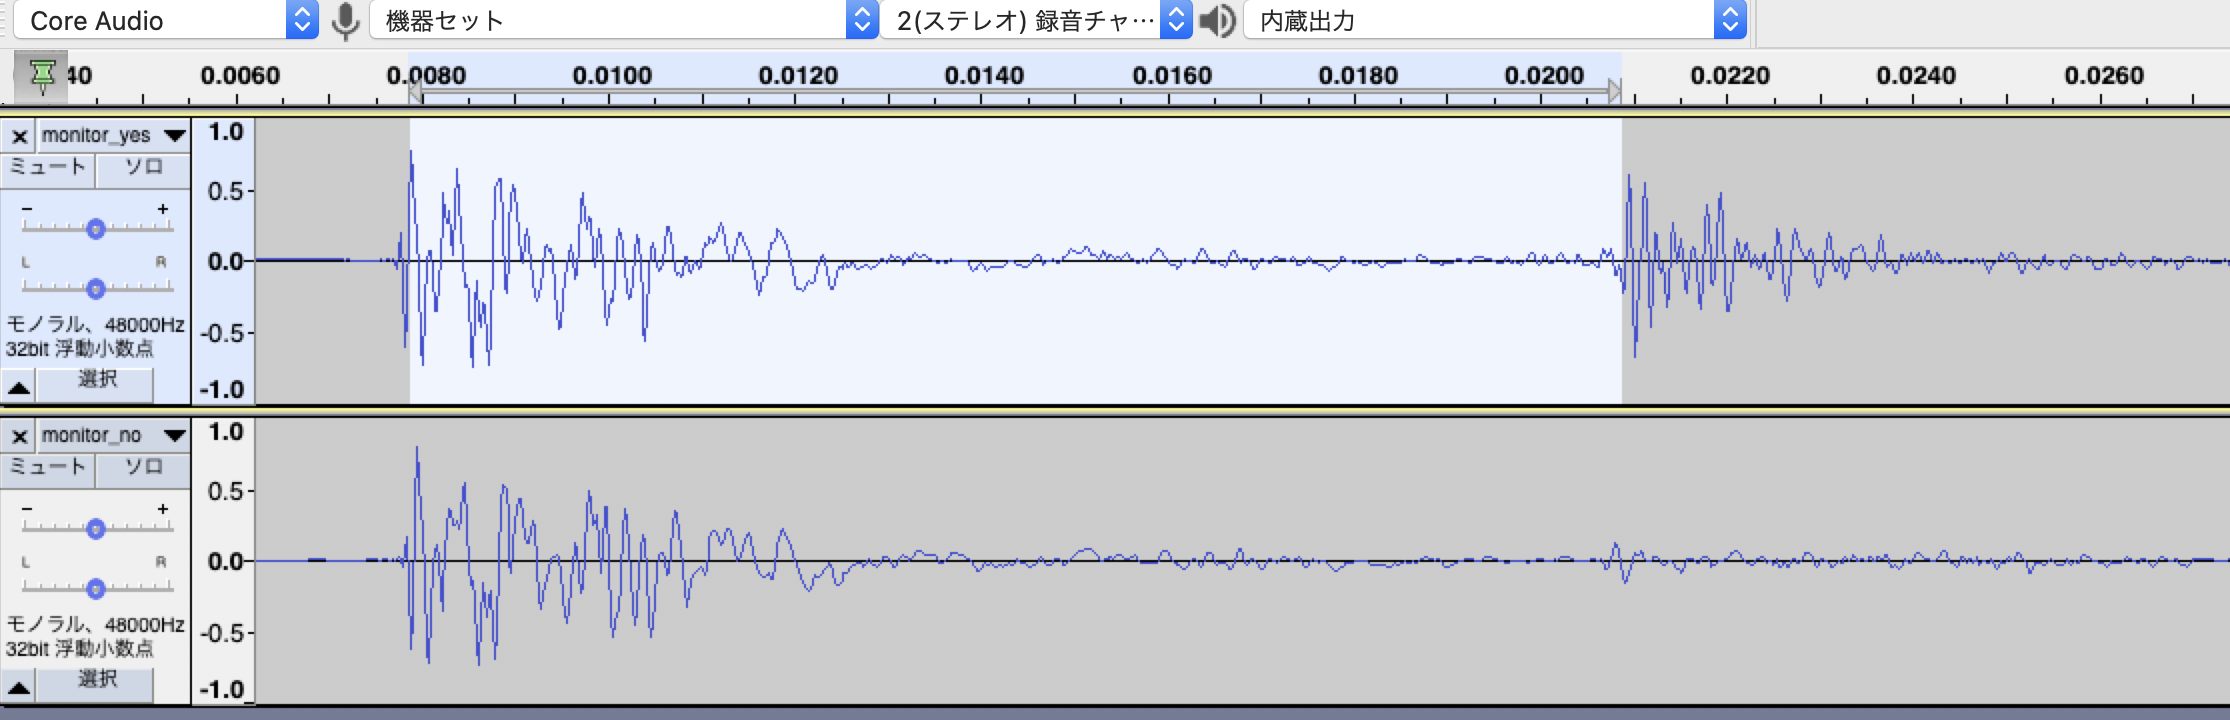
\includegraphics[width=\linewidth]{img/advance_test_monitor.png}
  \caption{Audacityで確認した録音ファイル}
  \label{fig:advance_test_monitor}
\end{figure}

\begin{figure}[tbp]
  \centering
  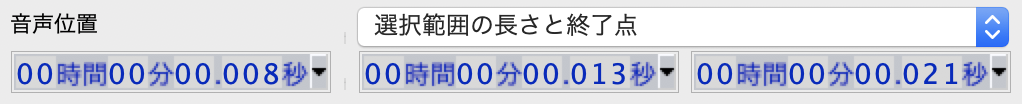
\includegraphics[width=\linewidth]{img/advance_test_monitor_length.png}
  \caption{選択した範囲の長さ}
  \label{fig:advance_test_monitor_length}
\end{figure}

\section{まとめ}

本節で行った測定では、送受信にかかる時間を測定したため計測時間を2分の1にすることで簡易的に片道にかかる伝送時間を推測することができる。1ミリ秒を超えた回数は8回あったが、片道で1ミリ秒(往復2ミリ秒)以上になる回数は2回であった。よって、DanteにおけるAES67モードの遅延許容時間の1ミリ秒を99.99933\%(299998/300000)達成することができた。

また、追加実験においてA/D、D/A変換に要する時間は今回実験した環境では13ミリ秒で行えることがわかった。往復の伝送にかかる2ミリ秒程度の時間と、A/D、D/A変換に必要な13ミリ秒をあわせて\ref{sec:pro_audio_requirement}節にある目標の20ミリ以内を達成することができた。

業務用オーディオでは完璧な伝送が求められるが、オーディオが数サンプル欠落する程度であれば受信側で知覚できないよう工夫することはできると考えられる。ソフトウェアによるIPオーディオ伝送は、ソフトウェア処理にかかる時間やネットワーク上に流れる他のパケットによる影響で遅延がゆらぐことは想定しておかなければならない。この実験で1ミリ秒以下での伝送を100\%に近いレートで行えたことは、ソフトウェアIPオーディオ伝送は業務用オーディオにおいて現実的なものであるという知見が得られた。
